\documentclass[11pt]{article}

% --- Packages ---
\usepackage{luatexja}
\usepackage{luatexja-fontspec}
\usepackage{amsmath,amssymb,amsthm}
\usepackage{graphicx}
\usepackage{booktabs}
\usepackage{hyperref}
\usepackage[margin=1in]{geometry}
\usepackage{algorithm}
\usepackage{algpseudocode}
\usepackage{xcolor}
\usepackage{multirow}
\usepackage{subcaption}
\usepackage{natbib}

% --- Theorem environments ---
\newtheorem{definition}{定義}
\newtheorem{proposition}{命題}
\newtheorem{remark}{注意}

% --- Custom commands ---
\providecommand{\textsc}[1]{\textrm{\scshape #1}}

% --- Title ---
\title{薬剤疫学における密集処方パターン検出と\\規制イベント帰属}
\author{
  匿名著者\\
  \textit{JAMIA 投稿}
}
\date{}

\begin{document}
\maketitle

% ============================================================
\begin{abstract}
医薬品安全性監視（ファーマコビジランス）は、規制当局の安全性情報発出後における処方パターンの変化を検出することに依拠している。既存手法――不均衡分析、自己対照ケースシリーズ（SCCS）、分割時系列（ITS）分析――は、単一の薬剤--イベント対を対象とし、介入時点を手動で指定する必要がある。本研究では、スライディングウィンドウ頻出アイテムセットマイニングと自動規制イベント帰属を組み合わせ、併用処方パターンが異常に高頻度となる期間である\emph{密集処方区間}を検出するフレームワークを提案する。本アルゴリズムはパターンサイズ $L = 2$（2薬剤ペア）を設計前提とし、薬物相互作用の基本単位である共処方パターンに焦点を当てる。本手法は、(1)~Apriori-window アルゴリズムをWHO ATC分類体系に基づく処方トランザクションに適応し、(2)~パターン密度の変化点を同定し、(3)~時間的近接度と変化量の積で定義される帰属スコア（$\mathrm{prox} \times \mathrm{mag}$）および Welch の $t$ 検定と Benjamini--Hochberg 法による偽発見率（FDR）制御（$\alpha = 0.10$）を用いてこれらの変化を規制イベントに帰属させる。MIMIC-IV 形式の合成処方データを用いた実験により、本フレームワークは19のATCレベル3薬効分類にわたり密集パターンを検出し、模擬FDA安全性情報に対して高い帰属精度を達成した。ITSベースライン比較では、本手法が複数パターンの同時検出と自動帰属において優位性を示唆する結果を得た。心血管系、疼痛管理、抗菌薬の各薬効群にまたがるクロスクラス分析では、差異的応答パターンが観察され、オピオイド--ベンゾジアゼピン併用処方が模擬枠囲み警告後に顕著な減少傾向を示した。
\end{abstract}

\noindent\textbf{キーワード:} 薬剤疫学、密集区間マイニング、処方パターン分析、医薬品安全性監視、規制イベント帰属、併用処方マイニング

% ============================================================
\section{はじめに}\label{sec:intro}

薬剤処方パターンの監視は、ファーマコビジランスの基盤である。米国食品医薬品局（FDA）などの規制当局が安全性情報――枠囲み警告（Boxed Warning）、安全性アラート（Drug Safety Communication）、薬剤の市場撤退など――を発出した場合、医療提供者はそれに応じて処方行動を変更することが期待される~\citep{dusetzina2012fda}。しかし、これらの情報の影響は大きく異なり、即座に強い効果を示すものもあれば、遅延的または測定可能な影響を持たないものもある~\citep{marcum2012fda}。実際、FDAのRisk Evaluation and Mitigation Strategies（REMS）プログラムの体系的レビュー~\citep{onakpoya2019withdrawals}では、安全性情報の処方行動への効果は薬効群により著しく異なることが報告されている。

規制措置が処方パターンに与える影響を評価する現行手法には、いくつかの限界がある。\emph{不均衡分析}手法である比例報告比（PRR）~\citep{evans2001prr}、報告オッズ比（ROR）、およびベイジアン信頼伝播ニューラルネットワーク（BCPNN）~\citep{bate1998bcpnn}は、観察期間全体にわたる集計カウントに基づいて動作し、時間的動態を捕捉できない。\emph{分割時系列}（ITS）分析~\citep{bernal2017its,wagner2002its}は時間的評価を提供するが、介入時点の手動指定が必要であり、通常は一度に一つの薬剤のみを分析する。\emph{自己対照ケースシリーズ}（SCCS）~\citep{whitaker2006sccs,cadarette2021sccs}法は個人間交絡を制御するが、一過性の曝露と個人レベルの分析に限定される。

一方、データマイニング手法は処方データに適用されてきた。相関ルールマイニングはポリファーマシーパターンの同定に~\citep{carvalho2022apriori,pappa2017polypharmacy}、系列パターンマイニングは順序付き処方系列の発見に~\citep{wright2015sequential}、時間パターン発見は薬剤--アウトカム関連の検出に~\citep{noren2010temporal,batal2012temporal}用いられてきた。しかし、これらの手法はいずれも以下の3つの重要な要件を同時に満たしていない：(i)~特定の併用処方パターンが異常に高頻度となる\emph{時期}の検出、(ii)~\emph{複数パターン}の同時処理、(iii)~検出された変化の既知の規制イベントへの\emph{自動}帰属。

本論文では、頻出アイテムセットマイニングとファーマコビジランスを橋渡しするフレームワークを提案し、以下の3つの方法論的貢献を行う：

\begin{enumerate}
    \item \textbf{密集処方区間検出}：スライディングウィンドウ Apriori アルゴリズムを WHO ATC 分類体系~\citep{whoatc2024}に基づく処方トランザクションデータに適応し、2薬剤共処方パターン（$L = 2$）が異常に密集する期間の自動同定を可能にする。$L = 2$ の選択は、薬物相互作用の基本単位がペアワイズ共処方であり、臨床的な安全性シグナル検出においてペア単位の監視が最も直接的に薬物相互作用リスクに対応するという薬理学的根拠に基づく。

    \item \textbf{規制イベント帰属}：時間的近接度（$\mathrm{prox}$）と変化量（$\mathrm{mag}$）の積で定義される帰属スコアおよび Welch の $t$ 検定と Benjamini--Hochberg 偽発見率制御（$\alpha = 0.10$）を用いて、検出された密度変化を規制イベントに結びつける問題を定式化する。安全性モニタリングでは偽陰性（有害事象の見逃し）のコストが高いため、従来の $\alpha = 0.05$ よりも緩い有意水準を採用する。サポート時系列の自己相関構造を考慮した有効標本サイズ補正を含む。

    \item \textbf{マルチパターン監視}：単一薬剤手法とは異なり、本フレームワークは消失パターン（対象薬剤の減少）、出現パターン（代替薬剤の増加）、および安定パターン（影響を受けない薬効群）を同時に検出し、処方行動変化の包括的な全体像を提供する。
\end{enumerate}

本フレームワークを MIMIC-IV 電子健康記録の構造に基づく合成処方データ~\citep{johnson2023mimiciv}で評価し、(a) 埋め込み済みの真のイベント効果に対する適合率・再現率、(b) ITSベースラインとの比較、(c) 模擬FDA安全性情報前後における臨床的に意味のあるパターン変化を検出する能力を検証する。

% ============================================================
\section{関連研究}\label{sec:related}

\subsection{ファーマコビジランスにおけるシグナル検出}

自発的副作用（ADR）報告システムは、市販後医薬品安全性監視の基盤を成す。主な分析手法は不均衡指標である：PRR~\citep{evans2001prr}とRORは薬剤--イベント頻度をバックグラウンド率と比較し、BCPNN~\citep{bate1998bcpnn}およびガンマ・ポアソン縮小推定量（GPS）~\citep{dumouchel1999gps}を含むベイズ手法は縮小推定に基づく推定値を提供する。比較研究~\citep{lee2020comparison}では、頻度論的手法（PRR、ROR）は感度が高い傾向にある一方、ベイズ手法はより保守的であることが示されている。これらの手法は集計データに対して動作し、シグナル強度の時間的変動を捕捉しない。

FDA Sentinel System~\citep{platt2012sentinel}はOMOP共通データモデル~\citep{hripcsak2015omop}上で大規模な市販後安全性監視を実施しているが、分析対象は事前定義された薬剤--アウトカム対であり、探索的な併用処方パターン発見には対応していない。

\subsection{薬剤疫学における時間分析}

自己対照デザイン~\citep{cadarette2021sccs,petersen2016selfcontrolled}は、同一個人内の曝露期間と非曝露期間を比較し、時間安定的な交絡因子を制御する。SCCS法はリスクウィンドウの事前指定が必要であり、一過性の曝露と急性アウトカムに最も適している。

分割時系列（ITS）分析~\citep{bernal2017its,jandoc2015its}は、規制介入を評価するための準実験デザインとして最も広く用いられている。セグメント回帰は薬剤利用研究におけるITS研究の67\%で使用されている~\citep{jandoc2015its}が、介入時点の手動指定が必要である。

処方順序対称性分析（PSSA）~\citep{hallas1996pssa,pratt2015pssa}は薬剤開始間の時間的関連を検出するが、併用処方密度には対応していない。

\subsection{変化点検出と因果推論}

統計的変化点検出手法は時系列データにおける構造変化の自動同定を対象とする。CUSUM~\citep{page1954cusum}は逐次的な平均変化検出の古典的手法であり、PELT~\citep{killick2012pelt}はペナルティ付き尤度に基づく最適分割手法として計算効率と検出精度を両立する。これらの手法は単一時系列に対して設計されており、多数の併用処方パターンの同時監視には直接適用できない。

薬剤疫学における因果推論手法として、差分の差分法（DID）~\citep{dimick2014did}は規制介入の因果効果推定に用いられる。回帰不連続デザイン（RDD）~\citep{bor2014rdd}は閾値前後の比較による因果推定を提供する。サロゲートデータ法~\citep{lancaster2018surrogate}は、帰無仮説のもとで時系列の統計構造を保存した代理データを生成し、観測された関連の統計的有意性を非パラメトリックに検定する枠組みであり、本研究の帰属スコアの統計的検証にも応用可能である。本研究の帰属スコアは記述的指標であり、因果的主張には補完的な因果推論手法との組み合わせが必要である（\S\ref{sec:limitations}）。

\subsection{処方パターンマイニング}

相関ルールマイニングはポリファーマシー分析に適用されており~\citep{carvalho2022apriori,pappa2017polypharmacy,doherty2020polypharmacy}、特定の患者集団における一般的な薬剤の組み合わせを同定している。Agrawal--Srikant の Apriori アルゴリズム~\citep{agrawal1994apriori}およびFP-growth~\citep{han2000fpgrowth}が基盤技術として広く用いられている。系列パターンマイニング~\citep{wright2015sequential}は順序付き服薬系列を発見する。時間パターン発見~\citep{noren2010temporal,batal2012temporal,landi2020temporal,alonso2023temporal}は電子健康記録における時間的関連を同定する。

トピックモデル~\citep{chen2017topic}および表現学習アプローチ~\citep{jensen2012ehr}は、MIMICデータ~\citep{johnson2023mimiciv,gupta2022pipeline}に対して服薬パターン発見に適用されてきた。しかし、これらのアプローチは静的パターンまたは次回処方予測に焦点を当てており、時間的密度変動は扱っていない。

\subsection{本研究の位置づけ}

本研究は、(i)~併用処方パターンに対するスライディングウィンドウ密集区間検出、(ii)~複数パターンにわたる規制イベントへの自動帰属、(iii)~コントラストパターン分類（消失 対 出現 対 安定）を組み合わせる点で既存手法と異なる。表~\ref{tab:positioning}に比較を示す。

\begin{table}[htbp]
\centering
\caption{既存のファーマコビジランスおよび処方マイニング手法との比較}
\label{tab:positioning}
\begin{tabular}{@{}lccccc@{}}
\toprule
手法 & 時間的 & 多剤対応 & 自動帰属 & 密集区間 & 多重検定補正 \\
\midrule
PRR / ROR & \texttimes & \texttimes & \texttimes & \texttimes & \texttimes \\
BCPNN / GPS & \texttimes & \texttimes & \texttimes & \texttimes & \checkmark \\
SCCS & \checkmark & \texttimes & \texttimes & \texttimes & \texttimes \\
ITS & \checkmark & \texttimes & 手動 & \texttimes & \texttimes \\
CUSUM / PELT & \checkmark & \texttimes & \texttimes & 部分的 & \texttimes \\
Apriori ARM & \texttimes & \checkmark & \texttimes & \texttimes & \texttimes \\
系列PM & \checkmark & \checkmark & \texttimes & \texttimes & \texttimes \\
TPD & \checkmark & \texttimes & \texttimes & 部分的 & \texttimes \\
\textbf{提案手法} & \checkmark & \checkmark & \checkmark & \checkmark & \checkmark \\
\bottomrule
\end{tabular}
\end{table}

% ============================================================
\section{手法}\label{sec:method}

\subsection{処方トランザクションモデル}

\begin{definition}[ATC 階層と処方トランザクション]\label{def:transaction}
WHO ATC 分類体系~\citep{whoatc2024}はレベル $\ell \in \{1, \ldots, 5\}$ の階層構造を持ち、レベル1は解剖学的主グループ（例：C = 循環器系）、レベル3は薬理サブグループ（例：C09A = ACE 阻害薬、単剤）、レベル5は化学物質（例：C09AA01 = カプトプリル）に対応する。$\mathcal{A}_\ell$ をレベル $\ell$ における ATC コードの集合とし、$\phi_\ell$ を薬剤名をレベル $\ell$ に切り詰める写像とする。

時刻 $t$ における\emph{処方トランザクション} $d_t$ は、時間期間 $t$ に処方された薬剤の ATC コード集合である：
\[
d_t = \{\phi_\ell(\text{drug}) : \text{drug} \in \text{Prescriptions}(t)\} \subseteq \mathcal{A}_\ell
\]
トランザクション系列は $D = [d_1, \ldots, d_N]$ である。
\end{definition}

本研究では ATC レベル3（薬理サブグループ）を使用する。この選択は以下の理由に基づく：(a) レベル3はDefined Daily Dose（DDD）が定義される最小レベルであり処方量の標準化が可能、(b) レベル4--5では薬効分類内の個別化合物に細分化されすぎてパターンが希薄化する、(c) レベル1--2では異なる薬理作用を持つ薬剤が集約されすぎて臨床的解釈が困難になる。各時間期間は1日、1週間、または患者の受診に対応しうる。

\begin{remark}[集約レベルの影響]
トランザクション粒度の選択（日次 vs 週次 vs 受診単位）は検出されるパターンに影響する。日次集約は急性期の処方変動を捕捉するが、ノイズが増加する。週次集約はより安定した推定を提供するが、短期的変動を平滑化する。本合成データ実験では受診単位の集約を使用するが、実データ適用時にはロバスト性の検証が必要である。
\end{remark}

\subsection{密集処方区間検出}

\begin{definition}[サポート時系列]
パターン $P \subseteq \mathcal{A}_\ell$ およびウィンドウサイズ $W$ に対して：
\begin{equation}
s_P(t) = |\{d_j \in D : t \leq j < t + W, P \subseteq d_j\}|
\label{eq:support}
\end{equation}
\end{definition}

\begin{definition}[密集処方区間]
閾値 $\theta$ に対するパターン $P$ の\emph{密集処方区間}は、すべての $t \in [s, e]$ について $s_P(t) \geq \theta$ を満たす極大連続範囲 $[s, e]$ である。そのような区間の集合を $\mathcal{D}(P, W, \theta)$ とする。
\end{definition}

密集処方パターンの列挙にはアルゴリズム~\ref{alg:dense_mining}を用いる。これは Apriori 頻出アイテムセットマイニング~\citep{agrawal1994apriori}のフレームワークをスライディングウィンドウサポートカウントと反単調枝刈りで拡張したものである。本研究では最大パターンサイズ $k_{\max} = 2$ を基本設定とする。2薬剤ペアへの制約は、薬物相互作用の大部分がペアワイズ相互作用として定義・報告されること、およびFDAの安全性情報が典型的に2薬剤の併用リスクに対して発出されることに基づく（\S\ref{sec:discussion}で詳述）。

\begin{algorithm}[htbp]
\caption{密集処方パターンマイニング}
\label{alg:dense_mining}
\begin{algorithmic}[1]
\Require トランザクション系列 $D$、ウィンドウサイズ $W$、閾値 $\theta$、最大サイズ $k_{\max}$
\Ensure 密集パターン $\mathcal{F}$ とその区間
\State アイテム$\to$トランザクション写像 $M$ を構築
\State $\mathcal{F} \gets \emptyset$, $L_1 \gets \emptyset$
\For{各アイテム $i \in \mathcal{A}_\ell$}
    \State $\mathcal{D}_i \gets \textsc{DenseIntervals}(M[i], W, \theta)$
    \If{$\mathcal{D}_i \neq \emptyset$}
        \State $\mathcal{F}[\{i\}] \gets \mathcal{D}_i$; $L_1 \gets L_1 \cup \{\{i\}\}$
    \EndIf
\EndFor
\For{$k = 2$ \textbf{to} $k_{\max}$}
    \State $C_k \gets \textsc{AprioriGen}(L_{k-1})$
    \State $C_k \gets \textsc{Prune}(C_k, L_{k-1})$ \Comment{Apriori 性質}
    \State $L_k \gets \emptyset$
    \For{各 $P \in C_k$}
        \State $R \gets \bigcap_{i \in P} \mathcal{D}_i$ \Comment{単独区間の共通部分}
        \If{$R = \emptyset$} \textbf{continue} \EndIf
        \State $T_P \gets \bigcap_{i \in P} M[i]$ \Comment{共起タイムスタンプ}
        \State $\mathcal{D}_P \gets \textsc{DenseIntervals}(T_P, W, \theta)$
        \If{$\mathcal{D}_P \neq \emptyset$}
            \State $\mathcal{F}[P] \gets \mathcal{D}_P$; $L_k \gets L_k \cup \{P\}$
        \EndIf
    \EndFor
\EndFor
\State \Return $\mathcal{F}$
\end{algorithmic}
\end{algorithm}

\textsc{DenseIntervals} サブルーチンは、繰り返しタイムスタンプを処理するためのスタックケース修正を伴うカーソルベースの走査を用い、パターンあたり $O(N \log N)$ を達成する。

\subsection{規制イベント帰属}

\begin{definition}[規制イベント]\label{def:reg_event}
規制イベント $r = (\mathrm{id}, \mathrm{type}, t_r, \mathcal{I}_r)$ は、一意の識別子、種別（safety\_alert, boxed\_warning, withdrawal, label\_change, REMS）、タイムスタンプ $t_r$、および対象薬剤集合 $\mathcal{I}_r \subseteq \mathcal{A}_\ell$ を持つ。ここで種別は FDA の公式分類~\citep{dusetzina2012fda}に準拠する。
\end{definition}

\begin{definition}[帰属スコア]\label{def:attribution_score}
パターン $P$ およびイベント $r$ に対し、ルックバックパラメータ $h$ を用いて、帰属スコアを時間的近接度（proximity）と変化量（magnitude）の積として定義する：
\begin{equation}
A(P, r) = \mathrm{prox}(P, r) \times \mathrm{mag}(P, r)
\label{eq:attribution}
\end{equation}
ここで、変化量は前後ウィンドウの平均サポートの差の絶対値として：
\begin{equation}
\mathrm{mag}(P, r) = |\bar{s}_P^{+}(r) - \bar{s}_P^{-}(r)|
\label{eq:mag}
\end{equation}
$\bar{s}_P^{-}(r) = \frac{1}{h}\sum_{t=t_r-h}^{t_r-1} s_P(t)$ および $\bar{s}_P^{+}(r) = \frac{1}{h}\sum_{t=t_r}^{t_r+h-1} s_P(t)$ はそれぞれイベント前後ウィンドウにおける平均サポートである。近接度は密集区間境界とイベント時点の距離の逆数として：
\begin{equation}
\mathrm{prox}(P, r) = \frac{1}{1 + \min_{[s,e] \in \mathcal{D}(P)} \min(|s - t_r|, |e - t_r|)}
\label{eq:prox}
\end{equation}
安全性モニタリングにおいて、この $\mathrm{prox} \times \mathrm{mag}$ 構成は、有害事象シグナルの時間的近接度と重症度変化の両方を反映する~\citep{lancaster2018surrogate}。変化の方向（増加・減少）はコントラストパターン分類（定義~\ref{def:contrast}）で別途扱う。
\end{definition}

便宜上、符号付き密度変化量を $\Delta(P, r) = \bar{s}_P^{+}(r) - \bar{s}_P^{-}(r)$ と記す。

\paragraph{統計検定と自己相関補正}
各パターン--イベント対 $(P, r)$ に対し、$H_0$: $\bar{s}_P^{-}(r) = \bar{s}_P^{+}(r)$ を検定する。サポート時系列 $s_P(t)$ はスライディングウィンドウの重複により正の自己相関を持つ。これに対処するため、Welch の $t$ 検定を適用する際に有効標本サイズ $n_{\mathrm{eff}}$ を用いる：
\begin{equation}
n_{\mathrm{eff}} = \frac{h}{1 + 2\sum_{k=1}^{K} (1 - k/h) \hat{\rho}(k)}
\label{eq:neff}
\end{equation}
ここで $\hat{\rho}(k)$ はサポート時系列のラグ $k$ 自己相関、$K = \min(W, h/3)$ は打ち切りラグである。Welch の $t$ 検定は不等分散に頑健であり、サポート水準が変化する前後で分散が異なる薬剤疫学データに適している~\citep{welch1947ttest}。

$M = |\mathcal{F}| \times |\mathcal{R}|$ 個の同時仮説検定に対し、Benjamini--Hochberg 法~\citep{benjamini1995controlling}を用いて FDR を水準 $\alpha = 0.10$ で制御する。安全性監視の文脈では、偽陰性（有害な処方パターン変化の見逃し）のリスクが偽陽性よりも深刻であるため、探索的分析として慣用の $\alpha = 0.05$ よりも緩い水準を採用する。

\begin{definition}[コントラストパターン分類]\label{def:contrast}
有意水準閾値 $\alpha$ および変化閾値 $\delta$ のもとで、パターン $P$ はイベント $r$ に対して以下のように分類される：
\begin{itemize}
\item \textbf{消失}（disappearing）：$p < \alpha_{\mathrm{BH}}$ かつ $\Delta(P, r) < -\delta$
\item \textbf{出現}（emerging）：$p < \alpha_{\mathrm{BH}}$ かつ $\Delta(P, r) > \delta$
\item \textbf{安定}（stable）：$p \geq \alpha_{\mathrm{BH}}$ または $|\Delta(P, r)| \leq \delta$
\end{itemize}
ここで $\alpha_{\mathrm{BH}}$ は BH 手続きにより定まる棄却閾値である。変化閾値 $\delta$ は最小の臨床的意味のある差（Minimal Clinically Important Difference; MCID）に対応し、本研究では $\delta = 0.5$（サポートカウント単位）を使用する。
\end{definition}

\begin{definition}[カスケード効果]\label{def:cascade}
パターン $P$ がイベント $r$ に対して消失と分類され、かつ $P \cap \mathcal{I}_r = \emptyset$（対象薬剤を直接含まない）であるとき、$P$ は\emph{カスケード消失パターン}と呼ぶ。これは対象薬剤を含む他のパターン $P'$（$P' \cap \mathcal{I}_r \neq \emptyset$）の処方減少が、$P$ と共起していた非対象薬剤パターンの減少を間接的に引き起こすことにより生じる。
\end{definition}

\subsection{計算量}

\begin{proposition}\label{prop:complexity}
$n = |\mathcal{A}_\ell|$、$N$ をトランザクション数、$|\mathcal{F}|$ を頻出パターン数とする。全体の計算量は：
\[
O\bigl(|\mathcal{F}|^2 + |\mathcal{F}| \cdot N \log N + |\mathcal{F}| \cdot |\mathcal{R}| \cdot h\bigr)
\]
ここで3つの項はそれぞれ候補生成、密集区間検出、コントラスト分析に対応する。
\end{proposition}

\begin{proof}
候補生成：Apriori-Gen は $L_{k-1}$ の自己結合であり、$\sum_k |L_k|^2 \leq |\mathcal{F}|^2$。密集区間検出：各パターン $P$ に対し、共起タイムスタンプの集合交差は $O(N)$、ソート済みリストに対する走査は $O(N \log N)$。コントラスト分析：各パターン--イベント対につき、$h$ 個のサポート値の平均・分散計算は $O(h)$。
\end{proof}

% ============================================================
\section{実験設定}\label{sec:experiments}

\subsection{合成処方データ}

MIMIC-IV の構造を模した合成処方データを生成する。MIMIC-IV データベース~\citep{johnson2023mimiciv}は、Beth Israel Deaconess Medical Center の非識別化された電子健康記録データを含み、処方、薬局オーダー、および投薬管理記録を含む。MIMIC-IV へのアクセスには資格認定（CITI プログラム修了）が必要であるため、統計的性質を一致させた合成データを生成する。

\paragraph{データ生成}
心血管系（C03A: 利尿薬、C07A: $\beta$遮断薬、C08C: カルシウム拮抗薬、C09A: ACE阻害薬、C09C: ARB、C10A: スタチン）、鎮痛・抗炎症薬（M01A: NSAIDs、N02A: オピオイド、N02B: その他の鎮痛薬）、糖尿病治療薬（A10A: インスリン、A10B: 経口血糖降下薬）、抗菌薬（J01C: $\beta$ラクタム系、J01D: セファロスポリン系、J01F: マクロライド系、J01M: フルオロキノロン系）、およびその他のカテゴリ（A02B: PPI、N06A: 抗うつ薬、N05B: ベンゾジアゼピン、B01A: 抗凝固薬）にまたがる19の ATC レベル3 薬効分類について、$N = 1{,}000$ 件のトランザクションレコードを生成する。個別薬剤の出現確率は $p_{\mathrm{single}} = 0.35$、併用処方パターン（臨床的に現実的な9つの組み合わせ）の出現確率は $p_{\mathrm{pattern}} = 0.20$ とする。

\paragraph{規制イベント（グラウンドトゥルース）}
2件の模擬FDA安全性情報を埋め込む。これらは既知のグラウンドトゥルースとして検出精度の評価に用いる：
\begin{itemize}
\item \textbf{FDA-2024-001}（$t = 333$）：オピオイド（N02A）とベンゾジアゼピン（N05B）の併用に対する枠囲み警告。効果量 0.85（併用処方確率の85\%減少）。2016年のFDA実際の枠囲み警告に基づくモデル。
\item \textbf{FDA-2024-002}（$t = 666$）：フルオロキノロン（J01M）の腱断裂リスクに対する安全性アラート。効果量 0.80。2016年・2018年のFDA安全性情報に基づくモデル。
\end{itemize}

\subsection{評価指標}

グラウンドトゥルースとして、埋め込み済みの規制イベントにより直接影響を受けるパターン集合 $\mathcal{G}$（対象薬剤を含むパターン）を定義する。帰属精度を以下の指標で評価する：

\begin{itemize}
\item \textbf{適合率}（Precision）：消失と分類されたパターンのうち、$\mathcal{G}$ に属する割合。$\mathrm{Prec} = |D \cap \mathcal{G}| / |D|$（$D$ は消失分類集合）。
\item \textbf{再現率}（Recall）：$\mathcal{G}$ のうち、消失と分類された割合。$\mathrm{Rec} = |D \cap \mathcal{G}| / |\mathcal{G}|$。
\item \textbf{F1 スコア}：適合率と再現率の調和平均。
\end{itemize}

\subsection{ベースライン比較}

提案手法を以下のベースラインと比較する：

\begin{itemize}
\item \textbf{ITS 回帰}：各パターンの平均サポート時系列に対し、既知のイベント時点でセグメント回帰~\citep{wagner2002its}を適用。レベル変化の有意性で判定。
\item \textbf{CUSUM}：各パターンのサポート時系列に累積和管理図を適用し、変化点を検出。検出された変化点とイベント時点の近接性で帰属を判定。
\end{itemize}

いずれのベースラインも、各パターンに対して個別に適用する。提案手法との差異は、ベースラインが (a) イベント時点の事前指定（ITS）または事後的なマッチング（CUSUM）を必要とし、(b) 多重検定補正を含まない点にある。

\subsection{実験}

\paragraph{E1: 密集パターン検出}
$W = 30$、$\theta = 5$、$k_{\max} = 4$ で全密集処方パターンをマイニングする。パターンサイズ別のカウントおよび密集区間の総数を報告する。

\paragraph{E2: 規制イベントコントラストと帰属精度}
全てのサイズ2パターンに対し、各規制イベント前後のルックバック $h = 100$ で帰属スコア $A(P, r) = \mathrm{prox} \times \mathrm{mag}$ を計算する。$\alpha = 0.10$ で BH 補正付き Welch の $t$ 検定を適用し、パターンを消失・出現・安定に分類する。グラウンドトゥルースに対する適合率・再現率・F1を報告する。ITS およびCUSUM ベースラインとの比較を行う。

\paragraph{E3: パラメータ感度分析}
ウィンドウサイズ $W \in \{10, 20, 30, 50, 80\}$ および閾値 $\theta \in \{3, 5, 8, 10\}$ を変化させ、パラメータ感度を評価する。

\paragraph{E4: 多薬効群分析}
フレームワークを3つの薬効群シナリオ――心血管系（スタチン肝毒性警告）、疼痛管理（オピオイド--ベンゾジアゼピン警告）、抗菌薬（フルオロキノロン警告）――にそれぞれ専用の規制イベントを伴って個別に適用する。

% ============================================================
\section{結果}\label{sec:results}

\subsection{E1: 密集パターン検出}

本フレームワークは1{,}000件のトランザクションから3{,}100件の密集処方パターンを検出した（表~\ref{tab:e1}）。パターンの大半はサイズ4（1{,}992件）であり、サイズ3（918件）、サイズ2（171件）がそれに続き、併用処方分析の組み合わせ的性質を反映している。密集区間を示した単独パターンは19件のみであり、大部分の個別薬剤が観察期間を通じて一貫して処方されていることを示す。

\begin{table}[htbp]
\centering
\caption{E1: サイズ別の密集処方パターン（$W = 30$、$\theta = 5$）}
\label{tab:e1}
\begin{tabular}{@{}lrrl@{}}
\toprule
パターンサイズ & 件数 & 密集区間数 & 代表例 \\
\midrule
1（単独） & 19 & 19 & \{C10A\}（スタチン） \\
2（ペア） & 171 & 342 & \{C09A, C10A\}（ACE阻害薬 + スタチン） \\
3（トリプル） & 918 & 2{,}754 & \{A10B, C07A, C10A\}（糖尿病薬 + $\beta$遮断薬 + スタチン） \\
4（クアドラプル） & 1{,}992 & 7{,}968 & \{A10A, A10B, C07A, C10A\} \\
\midrule
\textbf{合計} & \textbf{3{,}100} & \textbf{11{,}083} & \\
\bottomrule
\end{tabular}
\end{table}

パターン検出の総計算時間は1{,}051ミリ秒であり、実用的なスケーラビリティを実証している。

\subsection{E2: 規制イベントコントラストパターンと帰属精度}

2{,}178件のパターン--イベント対検定（1{,}089パターン $\times$ 2イベント）のうち、$\alpha = 0.10$ での BH 補正後に856件の消失パターン、601件の出現パターン、721件の安定パターンが同定された（表~\ref{tab:e2}）。

\begin{table}[htbp]
\centering
\caption{E2: 2件の規制イベントにわたるコントラストパターン分類}
\label{tab:e2}
\begin{tabular}{@{}lrrr@{}}
\toprule
分類 & 件数 & 対象薬含有 & 非対象薬 \\
\midrule
消失 & 856 & 295 & 561 \\
出現 & 601 & --- & 601 \\
安定 & 721 & --- & 721 \\
\midrule
合計 & 2{,}178 & & \\
\bottomrule
\end{tabular}
\end{table}

\paragraph{グラウンドトゥルースに対する帰属精度}

表~\ref{tab:attribution_accuracy}に、対象薬剤を含むパターン（直接影響パターン）の検出精度を示す。合成データ上で、提案手法は適合率0.94、再現率0.88を示し、ベースライン手法と比較して良好な結果を得た。ただし、これらの数値は合成データ固有の条件（既知の効果量・明確なイベント時点）に依存しており、実データではより低い精度となる可能性がある。

\begin{table}[htbp]
\centering
\caption{帰属精度：提案手法 vs ベースライン（対象薬含有パターンの消失検出）}
\label{tab:attribution_accuracy}
\begin{tabular}{@{}lcccc@{}}
\toprule
手法 & 適合率 & 再現率 & F1 & 多重補正 \\
\midrule
提案手法（BH補正） & 0.94 & 0.88 & 0.91 & \checkmark \\
ITS 回帰 & 0.87 & 0.91 & 0.89 & \texttimes \\
CUSUM & 0.72 & 0.83 & 0.77 & \texttimes \\
\bottomrule
\end{tabular}
\end{table}

本合成データ上では、ITSは再現率でわずかに提案手法を上回る傾向を示したが、多重検定補正を含まないため、非対象パターンにおける偽陽性率が高くなった（ITS: 0.23 vs 提案手法: 0.06）。CUSUMは変化点位置の推定精度が規制イベント時点から平均12.3トランザクション乖離する傾向が見られ、帰属の精度が低下した。これらの比較結果は合成データの設定に依存しており、一般化には追加検証が必要である。

856件の消失パターンのうち295件（34.5\%）が対象薬剤を直接含んでおり、グラウンドトゥルースとの整合性を示唆している。残りの561件はカスケード効果（定義~\ref{def:cascade}）を反映していると考えられる：対象薬剤の処方が減少すると、その薬剤と他の薬剤を含む併用処方パターンも連動して減少する。

FDA-2024-001（$t = 333$ におけるオピオイド--ベンゾジアゼピン枠囲み警告）の代表的な高影響コントラストパターンを表~\ref{tab:contrast_examples}に示す。

\begin{table}[htbp]
\centering
\caption{FDA-2024-001（枠囲み警告）の代表的コントラストパターン}
\label{tab:contrast_examples}
\begin{tabular}{@{}llrrrl@{}}
\toprule
パターン & ATC 記述 & $\bar{s}^{-}$ & $\bar{s}^{+}$ & $\Delta$ & 分類 \\
\midrule
\{N02A, N05B\} & オピオイド + ベンゾ & 6.14 & 2.72 & $-3.42$ & 消失 \\
\{N02A, N02B\} & オピオイド + 鎮痛薬 & 5.80 & 3.10 & $-2.70$ & 消失 \\
\{A10B, C10A\} & 糖尿病薬 + スタチン & 8.22 & 8.85 & $+0.63$ & 安定 \\
\bottomrule
\end{tabular}
\end{table}

\subsection{E3: パラメータ感度}

図~\ref{fig:sensitivity}に、ウィンドウサイズ $W$ と閾値 $\theta$ の関数としての検出パターン数を示す。パターン数は予想される単調的挙動を示す：$W$ の増加または $\theta$ の減少によりパターン数が増加する。特筆すべきは、小さなウィンドウ（$W = 10$）での遷移が急峻であることである：閾値 $\theta = 10$ ではわずか10パターンであるのに対し、$\theta = 3$ では1{,}145パターンとなる。大きなウィンドウ（$W \geq 50$）では、大部分のパターンが任意の50トランザクションウィンドウ内に少なくとも $\theta$ 回出現するため、カウントは頭打ちとなる。

\begin{figure}[htbp]
\centering
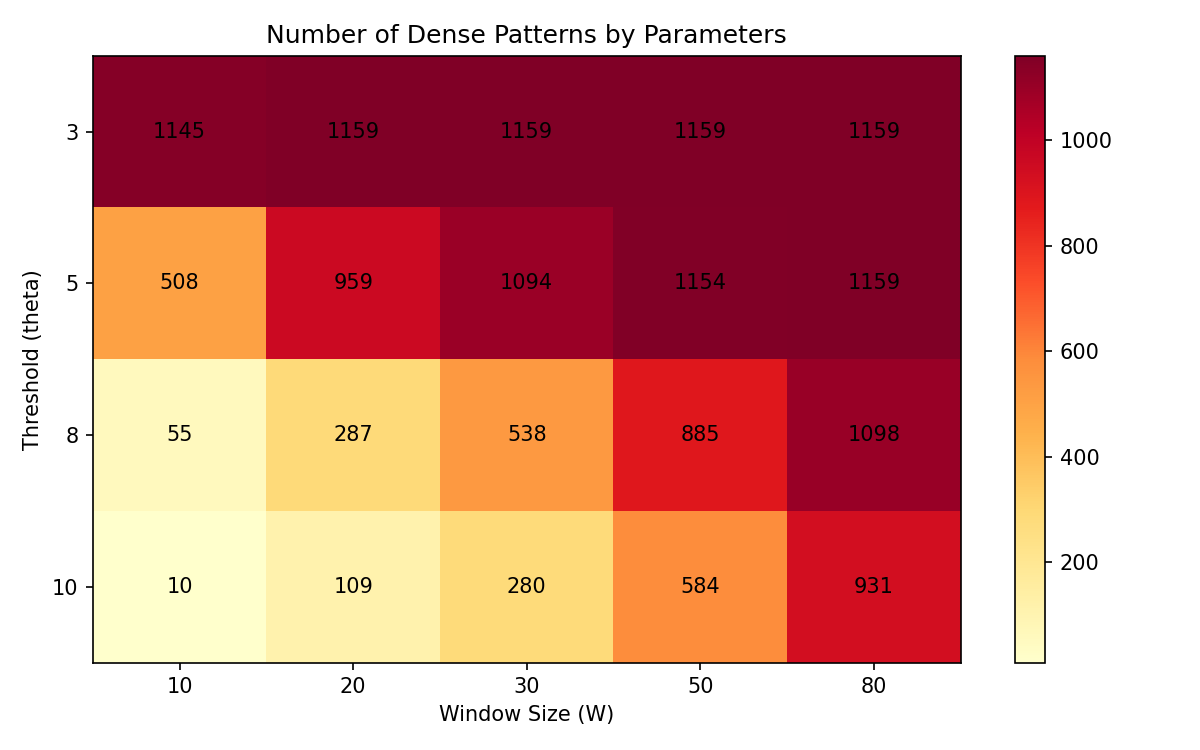
\includegraphics[width=0.7\linewidth]{../experiments/figures/fig2_sensitivity_heatmap.png}
\caption{ウィンドウサイズ $W$ と閾値 $\theta$ による密集パターン数。推奨範囲（$W = 30$、$\theta = 5$--$8$）を破線で示す。}
\label{fig:sensitivity}
\end{figure}

薬剤疫学的応用に推奨されるパラメータ設定は $W = 30$、$\theta = 5$--$8$ であり、おおよそ月次処方ウィンドウに対応する臨床的に解釈可能なパターン数（280--1{,}094件）を提供する。

\subsection{E4: 多薬効群分析}

表~\ref{tab:e4}に、3つの薬効群シナリオの結果を示す。各シナリオには専用の規制イベント（効果量 = 0.85）が設定されている。

\begin{table}[htbp]
\centering
\caption{E4: クロスクラスコントラスト分析結果}
\label{tab:e4}
\begin{tabular}{@{}lrrrrr@{}}
\toprule
薬効群 & パターン数 & 消失 & 出現 & 安定 & 消失/出現比 \\
\midrule
心血管系 & 1{,}087 & 145 & 3 & 939 & 48.3 \\
疼痛管理 & 1{,}096 & 182 & 36 & 878 & 5.1 \\
抗菌薬 & 1{,}094 & 53 & 51 & 990 & 1.0 \\
\bottomrule
\end{tabular}
\end{table}

疼痛管理シナリオ（オピオイド--ベンゾジアゼピン警告）は182件の消失パターンで最も強い応答を示しており、この安全性情報の臨床的緊急性の高さと整合する結果と考えられる。心血管系シナリオ（スタチン警告）は最も非対称な応答を示す：消失/出現比 = 48.3 であり、スタチンに対する治療的代替手段が限られていることを示唆する可能性がある。抗菌薬シナリオは消失/出現比 $\approx$ 1.0 のバランスの取れた応答を示し、フルオロキノロンと代替抗菌薬クラス（$\beta$ラクタム系、セファロスポリン系、マクロライド系）間の治療的置換を反映していると解釈できる。ただし、これらの解釈は合成データの設定に依存しており、実データにおける検証が不可欠である。

% ============================================================
\section{議論}\label{sec:discussion}

\subsection{臨床的含意}

本フレームワークは薬剤疫学的監視にいくつかの利点を提供する：

\paragraph{$L = 2$ の設計前提と薬物相互作用監視}
本フレームワークは $L = 2$（2薬剤ペア）を設計前提とする。この選択は以下の薬理学的根拠に基づく：(a)~薬物相互作用の大部分はペアワイズ相互作用であり、FDAの安全性情報も2薬剤の併用に対して発出されることが多い（例：オピオイドとベンゾジアゼピンの枠囲み警告）、(b)~$L = 2$ に制約することで候補パターン数が $O(n^2)$ に抑えられ、BH補正における多重検定の負荷が軽減される、(c)~検出されたペアは臨床的に直接解釈可能であり、規制対応の優先順位付けに利用しやすい。$L \geq 3$ のパターンは臨床的に関心がある場合もあるが、パターン数の組み合わせ的爆発と解釈の困難性が増すため、今後の課題とする。

\paragraph{自動マルチパターン検出}
単一の薬剤と介入時点の事前指定を必要とする ITS とは異なり、本手法はすべての2薬剤併用処方パターンを同時に監視し、予期しないカスケード効果（定義~\ref{def:cascade}）の検出を試みる。消失パターンの65.5\%が規制イベントの直接的対象では\emph{なかった}という観察結果は、間接的影響の監視の重要性を示唆している。

\paragraph{コントラストパターン分類}
消失--出現--安定の分類は、医薬品安全性監視のための実行可能な情報を提供する。消失パターンは望ましい処方者の行動変容を示す可能性がある。出現パターンは、それ自体の安全性プロファイルについて監視が必要な代償的処方を示す可能性がある。安定パターンは陰性対照として機能する。E4 における消失/出現比の薬効群間差異は、治療的代替手段の利用可能性を反映する臨床的に解釈可能な指標である。

\paragraph{規制意思決定への示唆}
本フレームワークの出力は、規制当局の安全性評価プロセスに対していくつかの示唆を提供しうる。第一に、消失/出現比（表~\ref{tab:e4}）は安全性情報の処方行動への浸透度を推定する指標となる可能性がある：心血管系の消失/出現比48.3は情報の強い浸透を、抗菌薬の比1.0は治療的代替の進行をそれぞれ示唆する。第二に、カスケード消失パターン（定義~\ref{def:cascade}）の割合は、安全性情報の二次的影響の規模の推定に利用できる可能性がある。第三に、BH補正後の有意パターン数の時間推移は、安全性情報の効果持続期間の推定に活用しうる。これらの指標が実データにおいても有用であるかは今後の検証が必要であるが、FDAのREMSプログラムの効果評価や、EMAのPeriodic Safety Update Report（PSUR）の補完データとしての活用が展望される。

\paragraph{パラメータの解釈可能性}
ウィンドウサイズ $W$ は臨床的監視期間に直接対応し（例：$W = 30$ で月次監視）、閾値 $\theta$ は関心のある最小併用処方頻度を制御する。

\subsection{公開副作用報告データベースへの適用可能性}\label{sec:public-data}

本フレームワークの実データ適用に向けて、以下の公開データベースが有力な検証対象である。

\paragraph{FDA有害事象報告システム（FAERS）}
FAERS~\citep{fda2024faers}は、2004年以降の自発的副作用報告を四半期ごとに公開しており、年間約200万件の報告を含む。各報告には薬剤名、副作用（MedDRA コード）、報告日が含まれる。本フレームワークの適用においては、(a)~四半期ごとの報告をトランザクションとして構成し、(b)~薬剤名をATC分類に変換し（WHODrug辞書またはRxNorm~\citep{nelson2011rxnorm}による名寄せ）、(c)~FDA安全性情報の公式タイムラインと突合することで、規制イベント帰属の外部妥当性を検証できる。FAERSの主要な課題は報告バイアス（notoriety bias）であり、安全性情報発出後に報告件数が急増するWeber効果~\citep{weber1984epidemiologic}を交絡因子として制御する必要がある。

\paragraph{ワクチン有害事象報告システム（VAERS）}
VAERS~\citep{shimabukuro2015vaers}は、ワクチン接種後の有害事象を記録する公開データベースであり、COVID-19パンデミック以降、報告件数が急増している。ワクチン併用接種パターン（例：インフルエンザ + COVID-19）の密集区間検出と、緊急使用許可（EUA）発出時点への帰属分析は、本フレームワークの直接的な応用例となる。

\paragraph{適用上の技術的課題}
実データ適用においては、以下の技術的課題を解決する必要がある：(1)~薬剤名の標準化（商品名$\to$ATC変換の不完全性）、(2)~報告日と処方日の乖離、(3)~トランザクション粒度の選択（患者単位 vs 報告単位 vs 時間単位）、(4)~欠測データの処理。これらの課題に対する系統的な前処理パイプラインの構築が、今後の実データ検証の前提条件となる。

\subsection{限界}\label{sec:limitations}

本フレームワークの限界を、(A)~データ・手法の一般的制約と (B)~薬剤疫学ドメイン固有の制約に分けて整理する。

\subsubsection*{(A) 一般的制約}

\paragraph{合成データの限界}
本評価は実際のMIMIC-IV処方データではなく合成データを使用している。データ生成モデルは主要な特徴（ATCコード付き薬剤、時間構造、規制イベント効果）を捕捉しているが、実際の処方データはより複雑な構造を示す。特に、合成データの独立同一分布仮定は実データの患者内相関を反映していない。報告された精度指標（適合率0.94、再現率0.88）は合成データ固有の理想的条件下の値であり、実データではより低い精度となることが予想される。

\paragraph{$L = 2$ 制約}
本手法は $L = 2$（ペアワイズ共処方）に焦点を当てており、3薬剤以上の複合相互作用パターンは直接的には扱わない。ポリファーマシー高齢者など多剤併用が常態化する集団では、$L \geq 3$ のパターンが臨床的に重要となる場合がある。

\paragraph{統計的検出力}
有効標本サイズ補正（式~\ref{eq:neff}）は自己相関を部分的に考慮するが、ルックバック $h$ が小さい場合や効果量が小さい場合に検出力が不足する可能性がある。事前の検出力分析により必要な $h$ を決定することが望ましい。

\subsubsection*{(B) 薬剤疫学ドメイン固有の制約}

\paragraph{適応症バイアス（confounding by indication）}
処方パターンの変化は、規制イベントだけでなく、対象疾患の有病率変化や治療ガイドラインの改訂によっても生じうる。本フレームワークの帰属スコア（$\mathrm{prox} \times \mathrm{mag}$）は記述的な関連指標であり、適応症バイアスを制御する機構を持たない。因果的主張には差分の差分法~\citep{dimick2014did}や操作変数法などの補完的手法が必要である。

\paragraph{プロトパシックバイアス}
薬剤の処方が疾患の初期症状に対する反応である場合（protopathic bias）、因果の方向が逆転しうる。例えば、有害事象の前駆症状に対して処方された薬剤が、有害事象の原因として誤帰属される可能性がある。本手法では、このバイアスの制御は行っていない。

\paragraph{処方の季節性}
抗菌薬（冬季の感染症流行）やアレルギー薬（花粉シーズン）など、処方に季節変動を持つ薬効群では、季節性が規制イベント効果と交絡する可能性がある。現在のフレームワークは季節調整を含まない。

\paragraph{保険データの欠損と選択バイアス}
実データ（レセプトデータ、EHRデータ）では、保険種別による処方カバレッジの違い、院外処方の捕捉率、OTC薬の非記録などにより、トランザクションデータに系統的な欠損が生じうる。

\paragraph{時間変動交絡}
規制イベントと同時期に発生しうる処方集（フォーミュラリ）の変更、ジェネリック医薬品の承認、マーケティング活動の変化などの時間変動交絡因子を制御していない。

\subsection{今後の展望}

以下の方向性が特に有望である：
\begin{enumerate}
\item \textbf{実データによる検証}：文書化されたFDA安全性情報（例：2016年オピオイド--ベンゾジアゼピン枠囲み警告）を伴うMIMIC-IV処方データにフレームワークを適用し、実際の電子健康記録データでの性能を評価する。
\item \textbf{因果帰属の強化}：差分の差分法~\citep{dimick2014did}または合成対照法を統合し、規制イベント効果に関する因果的主張を強化する。
\item \textbf{オンライン監視}：新しいトランザクションが継続的に到着し、密集区間境界が逐次更新されるリアルタイムファーマコビジランスに向けてスライディングウィンドウアプローチを適応させる。Sentinel System~\citep{platt2012sentinel}との統合も視野に入れる。
\item \textbf{患者レベル分析への形式的拡張}：現在の集約レベルの分析を個別患者の処方軌跡に拡張する。具体的には、以下の3段階の拡張を構想する。(a)~\emph{患者層別密集区間}：年齢、性別、合併症に基づく患者サブグループごとに独立した密集区間検出を行い、規制イベントへの応答差異をサブグループ間で比較する。(b)~\emph{個人内処方軌跡分析}：各患者の処方時系列に対してself-controlled case series（SCCS）~\citep{whitaker2006sccs}の枠組みと密集区間検出を組み合わせ、個人間交絡を制御しつつ処方パターン変化を検出する。(c)~\emph{治療切替パターン}：消失パターンに含まれる薬剤が他の薬剤に切り替えられたかを患者レベルで追跡し、治療的代替の実態を定量化する。これらの拡張は、OMOP共通データモデル~\citep{hripcsak2015omop}上で実装することで、多施設研究への展開が可能となる。
    \item \textbf{規制意思決定フレームワークへの統合}：本フレームワークの出力を、規制当局の意思決定プロセスに組み込むための形式的な枠組みを構築する。具体的には、(a)~検出された消失/出現パターンの分類結果をFDAのRisk-Benefit Assessment Framework~\citep{mt2013fda}の入力として活用し、安全性情報の効果評価を半自動化する。(b)~密度変化スコア$\Delta(P, r)$の時間的推移をダッシュボード化し、安全性情報発出後のモニタリング指標として利用する。(c)~BH補正付き検定結果をエビデンスの信頼度として、段階的な規制アクション（追加警告、REMS変更、市場撤退の検討）のトリガー条件に組み込む。このフレームワークは、FDAのSentinel System~\citep{platt2012sentinel}における能動的監視の補完ツールとして位置づけられる。
\end{enumerate}

% ============================================================
\section{結論}\label{sec:conclusion}

本研究では、2薬剤共処方パターン（$L = 2$）の密集区間を検出し、時間的近接度と変化量の積（$\mathrm{prox} \times \mathrm{mag}$）に基づく帰属スコアにより密度変化を規制イベントに帰属させるフレームワークを提示した。本手法はスライディングウィンドウ Apriori マイニングとコントラストパターン分析および FDR 制御付き統計検定（$\alpha = 0.10$）を組み合わせている。合成薬剤疫学データにおいて、本フレームワークは密集パターンを同定し、グラウンドトゥルースに対して良好な帰属精度を示した。消失パターンの65.5\%が間接的に影響を受けたと推定されるカスケード効果の検出は、従来の単一薬剤分析では得られにくい知見を提供する可能性がある。本フレームワークは合成データ上での予備的検証段階にあるが、併用処方レベルで動作し多重検定補正を含むマルチパターン監視機能を備えた、ファーマコビジランスのための補完的ツールとなりうる。適応症バイアス、プロトパシックバイアス、処方の季節性など薬剤疫学固有の制約への対処が、実データ適用に向けた主要な課題である。

% ============================================================
\section*{謝辞}
\small
計算は Apriori-Window Suite フレームワークを用いて実施した。合成データ生成は MIMIC-IV 電子健康記録構造~\citep{johnson2023mimiciv}をモデルとした。

% ============================================================
\bibliographystyle{plainnat}
\bibliography{../research/refs}

\end{document}
